%%% LaTeX Template: Two column article
%%%
%%% Source: http://www.howtotex.com/
%%% Feel free to distribute this template, but please keep to referal to http://www.howtotex.com/ here.
%%% Date: February 2011

%%% Preamble
\documentclass[	DIV=calc,%
							paper=a4,%
							fontsize=12pt,%
							onecolumn]{scrartcl}	 					% KOMA-article class

\usepackage{lipsum}													% Package to create dummy text
\usepackage[english]{babel}										% English language/hyphenation
\usepackage[protrusion=true,expansion=true]{microtype}				% Better typography
\usepackage{amsmath,amsfonts,amsthm}					% Math packages
\usepackage[pdftex]{graphicx}									% Enable pdflatex
\usepackage[svgnames]{xcolor}									% Enabling colors by their 'svgnames'
\usepackage[hang, small,labelfont=bf,up,textfont=it,up]{caption}	% Custom captions under/above floats
\usepackage{epstopdf}												% Converts .eps to .pdf
\usepackage{subfig}													% Subfigures
\usepackage{booktabs}												% Nicer tables
\usepackage{fix-cm}													% Custom fontsizes
\usepackage[utf8]{inputenc}
\usepackage[top=2.5cm, bottom=2.5cm, left=2.5cm, right=2.5cm]{geometry}
\usepackage[ddmmyyyy]{datetime}
\addto\captionsenglish{%
	\renewcommand\tablename{Tabela}
	\renewcommand\figurename{Figura}
} 
 

 
%%% Custom sectioning (sectsty package)
\usepackage{sectsty}													% Custom sectioning (see below)
\allsectionsfont{%															% Change font of al section commands
	\usefont{OT1}{phv}{b}{n}%										% bch-b-n: CharterBT-Bold font
	}

\sectionfont{%																% Change font of \section command
	\usefont{OT1}{phv}{b}{n}%										% bch-b-n: CharterBT-Bold font
	}



%%% Headers and footers
\usepackage{fancyhdr}												% Needed to define custom headers/footers
	\pagestyle{fancy}														% Enabling the custom headers/footers
\usepackage{lastpage}	

% Header (empty)
\lhead{}
\chead{}
\rhead{}
% Footer (you may change this to your own needs)

%% ====================================
%% ====================================
%% mude o rodape  do projeto
%% ====================================
%% ====================================

\lfoot{\footnotesize \texttt{Cabeamento estruturado} \textbullet ~Modelo de projeto}


\cfoot{}
\rfoot{\footnotesize página \thepage\ de \pageref{LastPage}}	% "Page 1 of 2"
\renewcommand{\headrulewidth}{0.0pt}
\renewcommand{\footrulewidth}{0.4pt}



%%% Creating an initial of the very first character of the content
\usepackage{lettrine}
\newcommand{\initial}[1]{%
     \lettrine[lines=3,lhang=0.3,nindent=0em]{
     				\color{DarkGoldenrod}
     				{\textsf{#1}}}{}}



%%% Title, author and date metadata
\usepackage{titling}															% For custom titles

\newcommand{\HorRule}{\color{DarkGoldenrod}%			% Creating a horizontal rule
									  	\rule{\linewidth}{1pt}%
										}

\pretitle{\vspace{-30pt} \begin{flushleft} \HorRule 
				\fontsize{50}{50} \usefont{OT1}{phv}{b}{n} \color{DarkRed} \selectfont 
				}

%% ====================================
%% ====================================
%% mude o titulo  do projeto
%% ====================================
%% ====================================

\title{Projeto de cabeamento estruturado}					% Title of your article goes here

%% ====================================



\posttitle{\par\end{flushleft}\vskip 0.5em}

\preauthor{\begin{flushleft}
					\large \lineskip 0.5em \usefont{OT1}{phv}{b}{sl} \color{DarkRed}}
\author{Anderson Vieira França}  	% Author name goes here


\postauthor{\footnotesize \usefont{OT1}{phv}{m}{sl} \color{Black} 
					\\Universidade Tecnológica Federal do Paraná - Câmpus Cornélio Procópio 								% Institution of author
					\par\end{flushleft}\HorRule}

\date{}																				% No date




%%% Begin document
\begin{document}
\maketitle
\thispagestyle{fancy} 	
\thispagestyle{empty}		% Enabling the custom headers/footers for the first page 
% The first character should be within \initial{}




%% ====================================
%% ====================================
%% mude o resumo  do projeto
%% ====================================
%% ====================================
\initial{E}\textbf{ste projeto de cabeamento estruturado foi desenvolvido para a empresa SCR, onde a mesma está construindo um novo escritório para atender seus clientes. Neste projeto consta todo o processo para a montagem do cabeamento assim como as plantas lógicas, física, topologia, encaminhamento dos cabos, cronograma de implantação, identificação dos cabos, plano de certificação, manutenção e custos.}

%% ====================================
\begin{figure}
	\centering
	
\includegraphics{utfpr}
\end{figure}

\vspace{3cm}
\centerline{\textit{\textbf{\today}}}

\clearpage
    \renewcommand*\listfigurename{Lista de figuras}
\listoffigures

\renewcommand*\listtablename{Lista de tabelas}
\listoftables




\clearpage
\renewcommand{\contentsname}{Sumário}
\tableofcontents
\clearpage

%% ====================================
%% ====================================
%% Inicio do texto
%% ====================================
%% ====================================
\section{Introdução}

O objetivo deste projeto é prover um projeto de cabeamento estruturado à empresa SCR. É  uma empresa que presta serviço realizando manutenções em microcomputadores. Está situada na região de Ibaiti/PR, com mais de dez anos de experiência no mercado. 

Este projeto de cabeamento estruturado tem como objetivo a definição da rede do novo escritório da empresa, onde será realizado o atendimento aos clientes.
\\

O novo escritório da empresa SCR conta com departamentos de recepção, atendimento ao cliente, comercial, SAC e gerência. A empresa possui atualmente onze colaboradores, sendo seis trabalhando no SAC, dois vendedores, uma no atendimento personalizado ao cliente, uma recepcionista e um gerente geral. Conta com cinco computadores notebooks, seis computadores desktops,  três  impressoras à laser e dois servidores, não possuindo equipamento de rede como switchs, roteadores, access point entre outros.  

\subsection{Benefícios}
O cabeamento estruturado oferece inúmeros benefícios desde que bem planejado, executado e administrando. O cabeamento estruturado tem por finalidade proporcionar um bom desempenho na estrutura da rede e uma base sólida provendo longevidade da rede. Permitindo flexibilidade na mudança do layout, diversos padrões físicos no meio físico, facilidade na manutenção, na substituição de equipamentos de rede e a documentação que permitirá a alteração e manutenção da estrutura de rede.
\\

Um dos grandes benefícios do cabeamento estruturado é a facilidade na identificação de erros na rede, manutenção mais rápida, melhor identificação de cabos e facilidade na instalação de novas estações de trabalho.

\section{Estado atual}
A empresa SCR não possui os equipamentos passivos e ativos de rede como cabos, patch panels e roteadores. Este projeto cobrirá todos os projetos de instalação do cabeamento e equipamentos necessários para a construção da rede estruturada desde os cabos, roteadores, switches de distribuição e conexão de rede dos departamentos.

\section{Usuários e Aplicativos}
Atualmente a empresa conta com onze colaboradores entre estes, seis estão alocados no setor de SAC. A empresa nos informou que em breve o número de colaboradores será maior. O setor de SAC Sistema de Atendimento ao Cliente é uma área fundamental para a empresa sendo necessária a contratação de mais colaboradores para melhor atendimento aos seus clientes.
\\

Outro setor que pode sofrer alterações no futuro é o de vendas, o qual poderá ser contratado mais vendedores para trabalho interno e externo na empresa. Com esses dados fornecidos é de extrema importância que o projeto seja realizado com a estimativa da evolução da empresa planejando os pontos de redes necessários atuais e futuramente.
 

\subsection{Usuários}
O quadro de colaboradores da empresa conta com onze colaboradores onde futuramente poderão ser contratadas mais oito pessoas para o sistema de atendimento ao cliente, três vendedores trabalhando internamente e externamente. Alguns usuários possuem o perfil de trabalho remoto onde será possível conectar ao sistema da empresa através do acesso remoto utilizando VPN em seus homes offices.

\subsection{Aplicativos}
A empresa SCR utiliza um sistema desenvolvido exclusivamente para suprir suas necessidades sendo de extrema importância o funcionamento 24 horas por dia. O sistema é utilizado para cadastro de seus clientes, fornecedores, contas a pagar e receber, relatórios de atendimentos, abertura de chamados via ticket ou e-mail.
\\

A disponibilidade do sistema de e-mail é fundamental para o funcionamento da empresa já que através dele são recebidos solicitação de atendimento e orçamentos. Todo atendimento da empresa é realizado através da telefonia IP, o departamento de SAC utiliza muito o sistema de telefonia para atender clientes, portanto é necessária uma rede estável e com capacidade de suprir todas as necessidades da empresa. 
\\

A contratação de um plano de internet dedicada com boa qualidade de download e upload se faz necessário para a utilização da VPN. Outro fator que faz necessário uma boa conexão com a internet é o fato que os atendentes do SAC realizam acesso remoto a desktop e servidores para realizar algumas configurações e manutenções de forma remota.


\section{Estrutura predial existente}
No layout da planta podemos verificar os setores existentes atualmente na empresa.


\begin{figure}
	\centering
	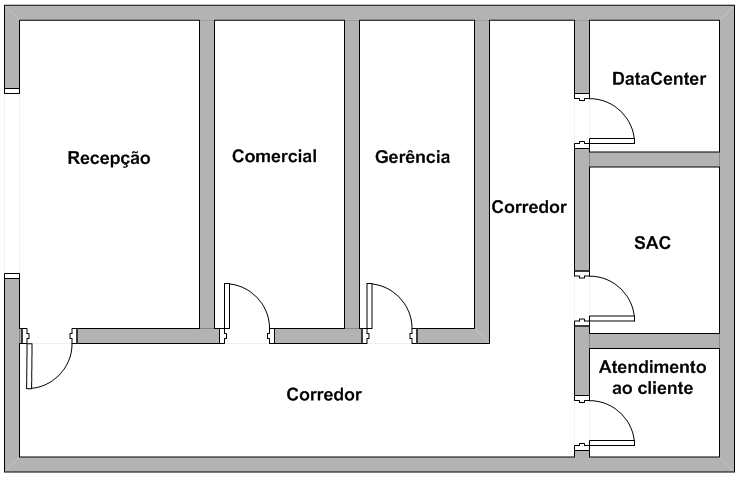
\includegraphics[height=\textwidth]{planta-baixa}
	\caption{Planta baixa}
	\label{planta-baixa}
	\end{figure}

Abaixo é apresentado o Layout junto com as distribuições dos equipamentos que serão utilizados.

\begin{figure}
	\centering
	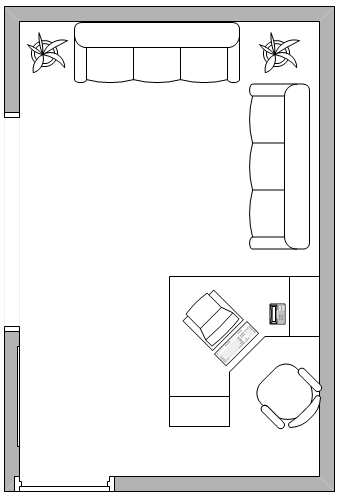
\includegraphics[height=\textwidth,angle=90]{recepcao}
	\caption{Recepção}
	\label{recepcao}
\end{figure}

\begin{figure}
	\centering
	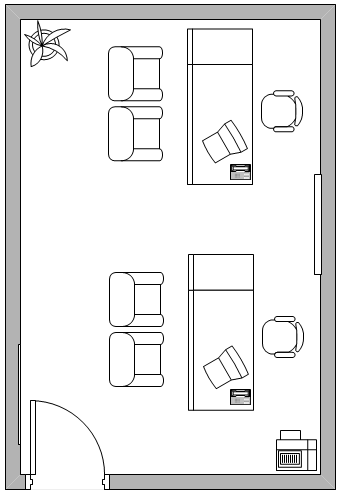
\includegraphics[height=\textwidth,angle=90]{comercial}
	\caption{Comercial}
	\label{comercial}
\end{figure}

\begin{figure}
	\centering
	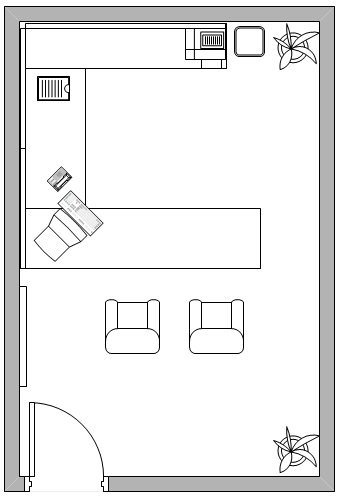
\includegraphics[height=\textwidth,angle=90]{gerencia}
	\caption{Gerência}
	\label{gerencia}
\end{figure}

\begin{figure}
	\centering
	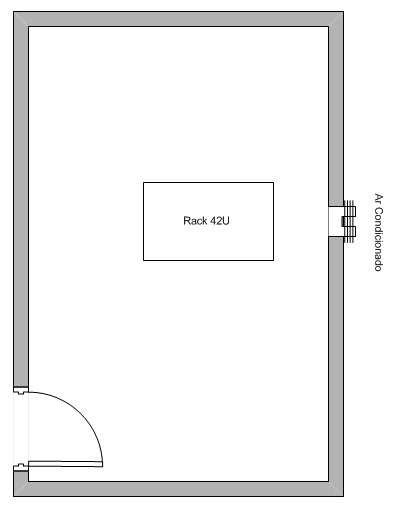
\includegraphics[height=\textwidth,angle=90]{datacenter}
	\caption{Datacenter}
	\label{datacenter}
\end{figure}

\begin{figure}
	\centering
	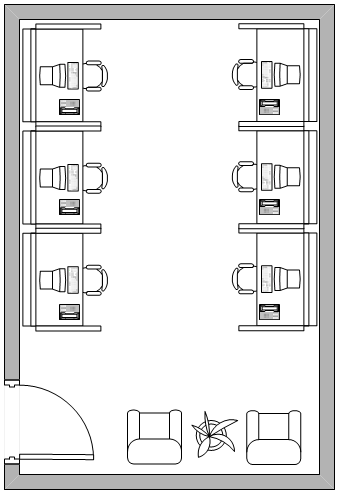
\includegraphics[height=\textwidth,angle=90]{sac}
	\caption{Sac}
	\label{sac}
\end{figure}

\begin{figure}
	\centering
	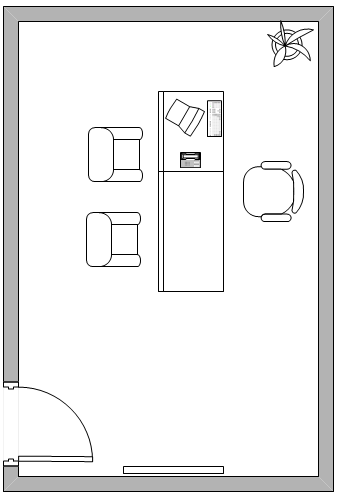
\includegraphics[height=\textwidth,angle=90]{atendimento}
	\caption{Atendimento}
	\label{atendimento}
\end{figure}

\section{Planta Lógica - Elementos estruturados}
Planta lógica com os devidos equipamentos e respectivas ligações lógicas.
\begin{figure}
	\centering
	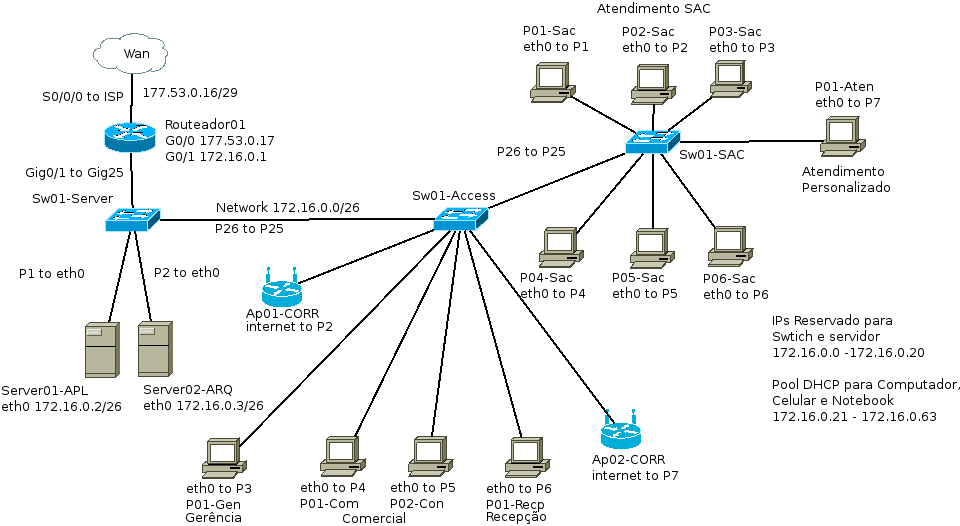
\includegraphics[height=\textwidth]{diagrama-logico}
	\caption{Diagrama lógico}
	\label{diagrama-logico}
\end{figure}

Abaixo está representada a tabela referente à rede utilizada e os endereços Ips de cada equipamento. Neste projeto foi utilizada uma máscara de rede /26, pois atualmente a rede possui poucos hosts, este dimensionamento da rede diminui o domínio de broadcast melhorando a desempenho da rede. Uma porcentagem dos 63 endereços na rede foram reservadas para atribuições em roteadores, servidores, access point e switch.
\\

O range de endereços 172.16.0.1 à 172.16.0.20 estão reservados para estes dispositivos. As estações de trabalho e celulares adquirem um endereço ip de forma dinâmica que é atribuído através do servidor de DHCP configurado no roteador central. O servidor de DHCP está configurado para atribuir o endereço IP a um determinado host analisando seu MAC Address assim sempre será atribuído o mesmo IP ao equipamento. O pool de DHCP abrange o range de 172.16.0.21 à 172.16.0.63.

\begin{figure}
	\centering
	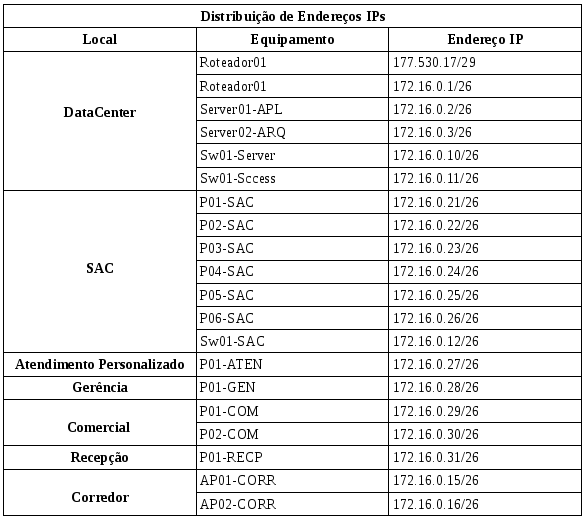
\includegraphics[height=\textwidth]{enderecos-ips}
	\caption{Distribuição de IPs}
	\label{enderecos-ips}
\end{figure}

\subsection{Diagrama de Rack}
Abaixo é mostrada o diagrama do rack após a instalção. 
\begin{figure}
	\centering
	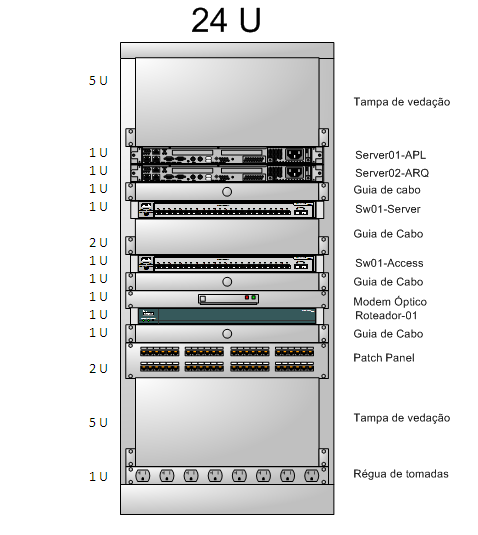
\includegraphics[height=\textwidth]{diagrama-rack}
	\caption{Diagrama de Rack Datacenter}
	\label{diagrama-rack}
\end{figure}

\begin{figure}
	\centering
	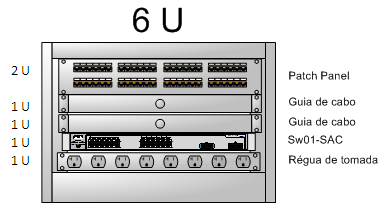
\includegraphics[height=\textwidth]{rack-sac}
	\caption{Diagrama de Rack Sac}
	\label{rack-sac}
\end{figure}

\subsection{Encaminhamento}

\begin{figure}
	\centering
	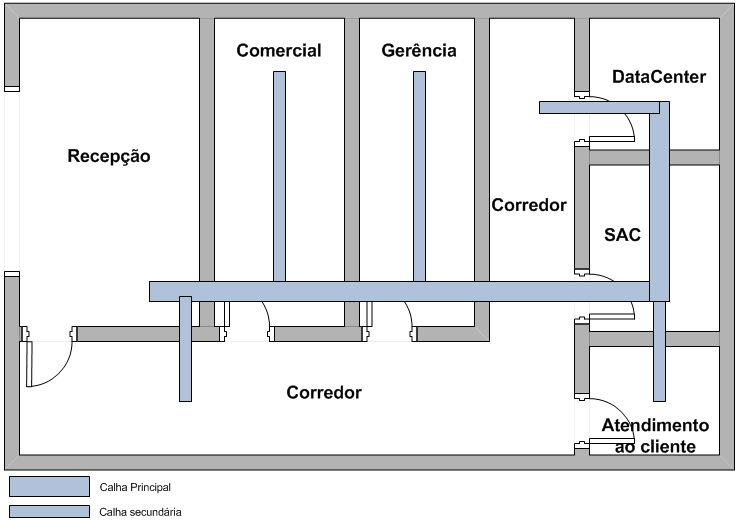
\includegraphics[height=\textwidth]{calha}
	\caption{Encaminhamento do Cabeamento}
	\label{calha}
\end{figure}

\subsection{Memorial descritivo}

\begin{figure}
	\centering
	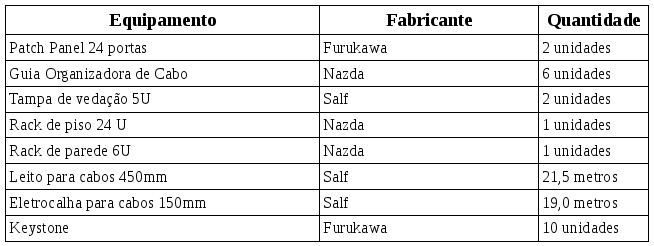
\includegraphics[height=\textwidth]{passivos}
	\caption{Equipamentos Utilizados}
	\label{passivos}
\end{figure}


\subsection{Identificação dos cabos}

\begin{figure}
	\centering
	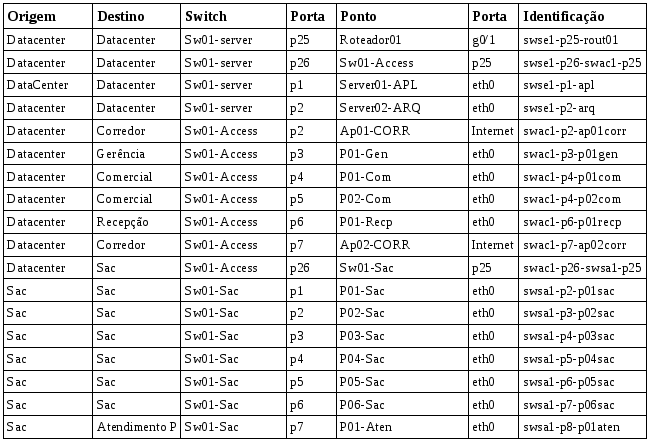
\includegraphics[height=\textwidth]{identificacao}
	\caption{Identificação dos Cabos}
	\label{identificacao}
\end{figure}

\section{Implantação}

\begin{figure}
	\centering
	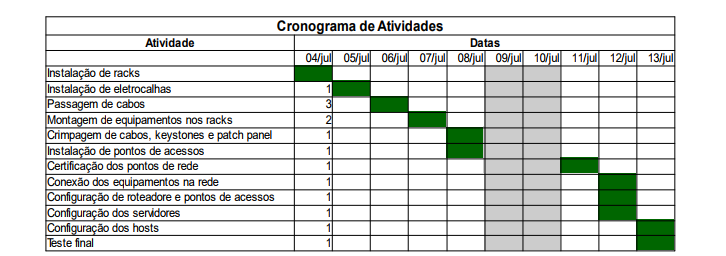
\includegraphics[height=\textwidth]{cronograma}
	\caption{Cronograma das Atividades}
	\label{cronograma}
\end{figure}


\section{Plano de certificação}

Após a instalação de toda parte física da rede será realizado a certificação de todos os pontos de redes deste o patch panel até a tomada fêmea na outra extremidade. O procedimento de certificação da rede abrange diversos parâmetros de testes como:
\begin{itemize}
	\item Perda de retorno (RL) 
	\item Perda de inserção (IL)
	\item Paradiafonia (NEXT)
	\item Relação de atenuação paradiafonia na extremidade próxima (ACRN)
	\item Relação de atenuação telediafonia (ACRF)
	\item Resistência em corrente contínua
	\item Desequilíbrio resistivo em corrente contínua
	\item Capacidade de transmissão de corrente
	\item Atraso de propagação
	\item Diferença de atraso de propagação
	\item Perda de conversão transversal e atenuação de acoplamento
\end{itemize}

Para a certificação é utilizado um analisador e certificador de cabos Fluke DTX-1800 e após os testes serão entregues a empresa contratante os relatórios em formato impresso e encadernados contendo todas as análises de cada ponto testado.

\section{Plano de manutenção}

O plano de manutenção preventiva compreende em manter a organização dos cabos, racks, patch panel. O plano de manutenção garante manter a identificação dos pontos de rede e atualização da documentação da rede.
\\

A cada noventa dias, será realizada uma inspeção técnica a fim de encontrar algum eventual problema no cabeamento, corrigir eventuais falhas, a realização de mudanças de pontos de rede e a ativação e certificação de novos pontos.

\subsection{Plano de expansão}
A empresa SCR não forneceu alguma intenção de expansão da rede prevista para os próximos doze meses. De qualquer forma o cabeamento estruturado permite a instalação de novos pontos em qualquer local da empresa onde passam ser necessários. O cabeamento da rede realiza um trajeto estratégico para poder adicionar novos pontos em qualquer departamento da empresa.


\section{Orçamento}

\begin{figure}
	\centering
	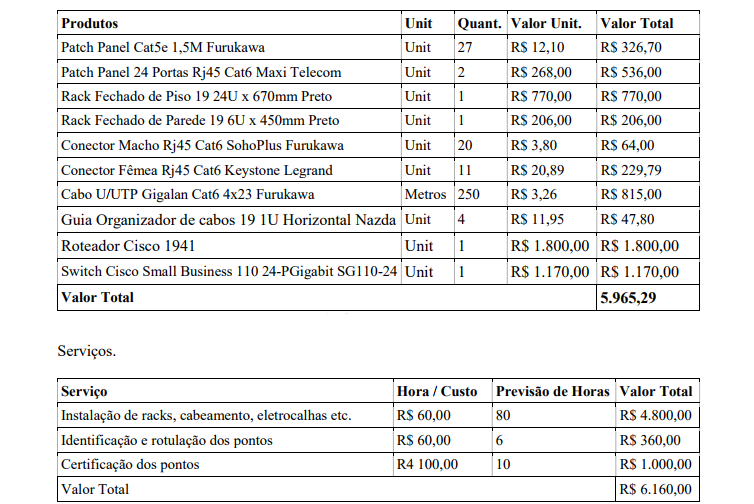
\includegraphics[height=\textwidth]{orcamento}
	\caption{Orçamento}
	\label{orcamento}
\end{figure}


\section{Referências bibliográficas}
MARIN, Paulo Sérgio. Cabeamento Estruturado - Desvendando cada passo: do Projeto à
Instalação. 1 ed. São Paulo: Érica, 2008. 336 p.
\\

PINHEIRO, José Mauricio S. Guia Completo de Cabeamento de Redes. 1 ed. Rio de Janeiro:
Campus, 2003. 264 p. 




%% ***********************************************************************
%% === remover daqui =====================================================
%% ***********************************************************************



%% ***********************************************************************
%% === ate aqui    =====  ================================================
%% ***********************************************************************
\end{document}\grid
